\section{Sinchroninės (angl. “synchronous”) integracijos}

\subsection{Sinchroninių integracijų principas}
Sinchroninės integracijos dar gali būti apibūdinamos kaip „dviejų žmonių komunikavimas realiu laiku“ \cite{Bk6}. Su sinchroniniais komunikavimo pavyzdžiais dažnai susiduriame visi. Vienas iš tokių yra apsilankymas paprastoje internetinėje svetainėje.
Interneto naršyklėje suvedus puslapio pavadinimą, HTTP protokolo pagalba, mums iš serverio yra užkraunamas svetainės turinys ir atvaizduojamas.
Šis komunikavimo būdas yra paremtas užklausos/atsakymo (angl. \textit{„request/response“}) principu. Šiame modelyje egzistuoja
Klientas (tai yra mūsų naršyklė) ir serveris (tai yra interneto svetainės savininkas arba įmonė teikianti svetainių talpinimo paslaugas).
Klientas siunčia užklausą serveriui prašydamas resurso, šiuo atveju tai yra mūsų norimos pamatyti svetainės turinio, ir laukia kol svetainė atiduos atsakymą į užklausą.
Serveris reaguodamas į kliento užklausą grąžina atsakymą, kuris būti arba svetainės turinys, arba grąžinama klaida, pavyzdžiui kad toks resuras neegzistuoja arba 
klientas yra neautorizuotas šios svetainės lankytojas. Šis bendravimas yra perteiktas pateikta schema (\ref{img:synchronous_model} pav.):

\begin{figure}[H]
  \centering
  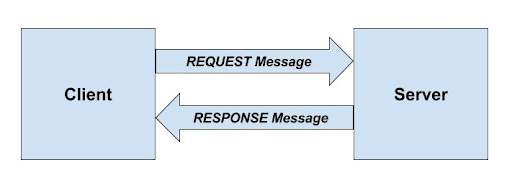
\includegraphics[scale=0.6]{img/synchronous_model}
  \caption{Sinchroninio komunikavimo schema.}
  \label{img:synchronous_model}
\end{figure}

Taigi šis modelis puikiai gali veikti ir mikroservisų sistemoje. Vienas servisas siunčia užklausą į kitą servisą norėdamas gauti
informaciją arba inicijuoti, kokį nors veiksmą. Šis modelis ypatingas tuo, kad yra primityvus ir iškart užklausą išsiuntęs servisas
žinos ar sėkmingai pavyko atlikti norimą veiksmą. Šis modelis yra labai geras, kai tik įvykus sėkmingai užklausai leidžiame vartotojui vykdyti
kitas operacijas ir kitaip bendrauti su mūsų sistema, tai yra vartotojo autentifikacija ir autorizacija.

\subsection{Sinchroninių integracijų technologijų tipai}
Būdų realizuoti sinchroninius komunikavimo modelius yra daug. Šiuo metu populiariausi yra du:
\begin{itemize}
	\item RESTful saityno tarnybos.
	\item SOAP saityno tarnybos.
\end{itemize}
\break

Turint omenyje, kad REST yra tik architektūrinis stilius, o ne protokolas, ir ju nelabai galima lyginti \cite{Misc5}. Tačiau
remiantis Joni Makkonen magistrinio darbo „REST ir SOAP saityno tarnybų efektyvumo ir naudojamumo palyginimas“ \cite{MstrThs2} galima teigti, kad
REST yra pranašesne ir šiame darbe išsiplėsime tik su šiuo architektūriniu stilium.
\break

REST saityno tarnybos užklausos struktūra yra paprasta. Ji susideda iš keletos atributų:
\begin{itemize}
	\item HTTP metodo, pvz.: \textit{„GET“, „POST“, „PUT“, „DELETE“}.
	\item Unikalaus resurso identifikatoriaus (arba adreso), pvz.: \textit{„http://mif.vu.lt/“}.
	\item Antraščių (angl. \textit{„Headers“}), pvz.: \textit{„Content-Type: application/json“}.
	\item Užklausos turinio (čia gali būti bet koks standartinis formatas, pvz.: \textit{„JSON“}).
	\item HTTP protokolo versija, pvz.: \textit{„HTTP/1.1“}.
\end{itemize}

REST atsakymo struktūra skiriasi nuo užklausos tik tuo, kad vietoje HTTP metodo, gaunamas HTTP statuso kodas. Tokio komunikavimo
per REST saityno tarnybas pavyzdį galime pamatyti šioje schemoje (\ref{img:Restful-scheme} pav.):

\begin{figure}[H]
  \centering
  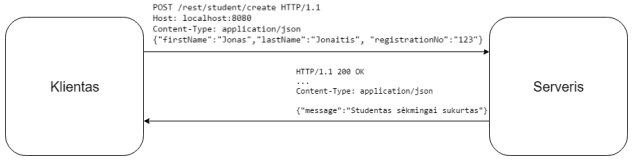
\includegraphics[scale=0.6]{img/Restful-scheme}
  \caption{REST saityno tarnybų schema.}
  \label{img:Restful-scheme}
\end{figure}

